\documentclass[12pt]{article}
\usepackage[english]{babel}
\usepackage[utf8x]{inputenc}
\usepackage[T1]{fontenc}
\usepackage{scribe}
\usepackage{listings}
\usepackage{wrapfig}
\usepackage{float}
\usepackage{booktabs}

\Scribe{Group 15 and Group 16}
\Lecturer{Abir De}
\LectureNumber{8}
\LectureDate{September 1, 2022}
\LectureTitle{Classifiers and Loss Functions, Tutorial 1 Solutions}

\lstset{style=mystyle}

\begin{document}
	\MakeScribeTop

%#############################################################
%#############################################################
%#############################################################
%#############################################################

\section{Classifiers}
Suppose we are given two datasets - $\calD_{\textrm{Train}} = \{\calX \times \calY\}^M$ and $\calD_{\textrm{Test}} = \{\calX \times \calY\}^N$. Here $\calX \subset \R^d$ is a set consisting of $d$-dimensional input features, while $\calY \subset \R$ consists of the corresponding labels.

The true classifier $h^*$ satisfies $h^*(x_j) = y_j$ for all $(x_j, y_j) \in \calD_{\textrm{Test}}$. On the other hand, we develop a classifier $\widehat{h}$ using only the training dataset, satisfying $\widehat{h}(x_i) = y_i$ for all $(x_i, y_i) \in \calD_{\textrm{Train}}$. Our aim is to find the best classifier $\widehat{h}$ which can mimic the true classifier $h^*$.

\section{Types of Classifiers}
\subsection{Complex $\widehat{h}$}
The most obvious classifier is simply a dictionary for $\calD_{\textrm{Train}}$, i.e. a {\bf Table Look-up} function. Here, we remember the label of each $x_i \in \calX_{\textrm{Train}}$ in our classifier $\widehat{h}$.  However, even though this can represent any function, this classifier will behave terribly on unseen data from the test set, on which we have no prior information about the label. Another disadvantage is that, as the data complexity of the dataset itself increases, storage and maintenance of this type of classifier can become cumbersome. Hence, we discard this classifier.

\subsection{Modest $\widehat{h}$}

\subsubsection{Voronoi classifier}

Another class of non-parametric classifiers consists of those using nearest neighbors. For example, the {\bf Voronoi classifier} involves making a convex polyhedron (called the Voronoi Cell) for each point in the training dataset and then finding the polyhedron in which a new data point lies.
\begin{figure}[h]
    \begin{center}
        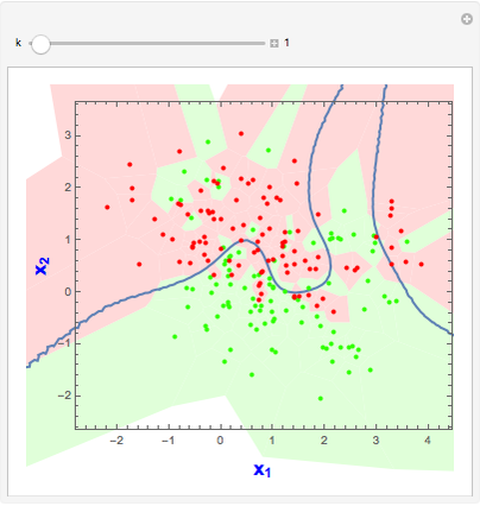
\includegraphics[width=0.6\textwidth]{knn.png}
        \caption{$1$-NN classifier for data with 2 classes}
        \label{fig:knn}
    \end{center}
\end{figure}
\subsubsection{{ Exhaustive $k$-Nearest Neighbor classifier}}


Another example is an {\bf Exhaustive $k$-Nearest Neighbor classifier}. Here, $k$ is a hyperparameter and not a learnable parameter. The idea is, for each new test data point, find the $k$ nearest neighbors from the training data, and give the majority class of these $k$ points. Note that this does not require any processing of the training data, and so the training time is negligible (probably the only $\calO(0)$ training time classifier we would see).

The benefit of the $k$-NN algorithm is that it works nicely with non-linear data. However, during inference, we have to find the $k$ nearest neighbors, which causes linear time blowup (time complexity will be of order $nd+n\log k$). This is undesirable in most situations, as we generally want testing to be fast so that the user does not have to wait for a long duration. Thus, we now move on to parameterised algorithms.

\subsection{Simple $\widehat{h}$}
A simple function for the classifier is the linear function, i.e. $\widehat{h} = w^Tx+b$. Note that this classifier may not work suitably for all possible datasets, and if the given dataset is highly non-linear, then this classifier would perform poorly.

\myfig{1}{linear.png}{Linear v/s Non-linear data}{fig:linear}

\subsubsection{Constant $\widehat{h}$}
A possible restriction to linear classifiers is the set of constant classifiers. The best constant classifier $\widehat{h} = c^*$ is given by $$c^* = \arg \min_c \sum_{(x_i,y_i) \in \calD_{\textrm{Train}}} \mathbb{I}[c \neq y_i]$$
This can easily be found as the mode label (also known as majority class) of the training data. However, although this classifier is easy to learn, it can perform poorly in the case when the distribution of the training data and the test data differs even slightly.
\newline \newline
So our focus is mostly on linear classifiers. Note that we don't go to higher dimensions (like quadratic functions), since the problem at hand is already pretty hard.

\subsection{Hypothesis Class}
The hypothesis class is the set of classifiers over which we are searching for the optimal. For example, for a linear classifier, this class is given by all possible linear functions, i.e. all possible pairs $(w,b)$ with weight $w \in \R^d$ and bias $b \in \R$.

\section{Error}
For any classifier $\widehat{h}$, the error that we aim to minimize is given by $$\textrm{Error}(\widehat{h}) = \sum_{(x_j,y_j) \in \calD_{\textrm{Test}}} \mathbb{I}[\widehat{h}(x_j) \neq y_j]$$
Our aim is to minimize the test error, but our classifier must be learned from the training dataset. In particular, the best classifier $h^*$ satisfies $$h^* = \arg \min_{\widehat{h} \in H} \sum_{(x_i,y_i) \in \calD_{\textrm{Train}}} \mathbb{I}[\widehat{h}(x_i) \neq y_i]$$

Note that, if the set of classifiers over which we are looking is not exhaustive enough, i.e. we are missing some crucial classifiers, then the error for any classifier in $H$ will be extremely large. So our hypothesis class should be able to generalize on $\calD_{\textrm{Test}}$.

\subsection{Linear Hypothesis Class}
Our aim is to find the optimal pair $\{w^*, b^*\}$ such that $$\{w^*, b^*\} = \arg \min_{w \in \R^d, \text{ } b \in \R} \sum_{i = 1}^M \mathbb{I}[w^Tx_i+b \neq y_i]$$
However, since we are searching over all $w \in \R^d$ and $b \in \R$, $w^Tx_i+b$ is a continuous function, which means that its probability of actually becoming exactly equal to a real number $y_i$ is $0$. In such a situation, the above error will become $M$ with probability $1$. Thus, we must change our error function.

\subsection{Discrete error - Based on Signum Function}
Let's assume that there are only $2$ classes, $-1$ and $1$, i.e. for all $1 \leq i \leq M$, we have $y_i \in \{-1, 1\}$. One option is to make our prediction $1$ if $w^Tx_i+b$ is non-negative, and $-1$ otherwise. This can be written as the classifier $h(x_i) = \sign(w^Tx_i+b)$. Thus, we wish to find the parameters $$\{w^*, b^*\} = \arg \min_{w \in \R^d, \text{ } b \in \R} \sum_{i = 1}^M \mathbb{I}[\sign(w^Tx_i+b) \neq y_i]$$
Note that the set $\calD_{\textrm{Train}}$ is {\bf scarce} (does not cover a lot of data points), so any discrete classifier will not be able to generalize well over the test set. Hence, it is better to look for {\bf probabilistic classifiers}. Another problem with a discrete classifier is that it will not be possible to find derivatives, which are required during gradient descent.

\subsection{Final Proposal for Error - Based on Sigmoid Function}
To mimic the discrete classifier, we replace the signum function with the sigmoid function. So our classifier will give the prediction $f(x_i) = \dfrac{1}{1+e^{-w^Tx_i+b}}$. Now we are looking for the parameters $$\{w^*, b^*\} = \arg \min_{w \in \R^d, \text{ } b \in \R} \sum_{i = 1}^M \mathbb{I}\left[\dfrac{1}{1+e^{-w^Tx_i+b}} \neq \dfrac{y_i+1}{2} \right]$$
Since the sigmoid function squeezes our prediction between $0$ and $1$, we have also changed the true prediction $-1$ to $0$, by shifting $y_i \longrightarrow \dfrac{y_i+1}{2}$.

Finally, the error function is still discrete, and so we replace it with a continuous function, giving the final classification problem proposal: $$\boxed{\{w^*, b^*\} = \arg \min_{w \in \R^d, \text{ } b \in \R} \sum_{i = 1}^M \max\left(0, \left(\dfrac{1}{2} - f(x_i) \right)y_i \right)}$$

\section{Solutions to Tutorial 1}
Presented below are the solutions to the first tutorial:

\subsection{Problem 1}

A loss function is a good approximator of $\mathbb{I}[\sign(h(x_i)) \neq y_i]$ if it takes a high value when $y_i$ and $h(x_i)$ are of different signs, while it is close to $0$ when they have the same sign.

\begin{wraptable}{R}{4cm}
\vspace{-1.5cm}
\begin{tabular}{ccc} \\ \toprule
y & h(x) & Loss \\ \midrule
+1 & > 0 & 0 \\ \midrule
-1 & > 0 & > 0 \\ \midrule
+1 & < 0 & > 0 \\ \midrule
-1 & < 0 & 0 \\ \bottomrule
\end{tabular}
\end{wraptable} 

\subsubsection{Part (i)}
 
      max\{0, 1 - y_i\cdot h(x_i)\}\ \ \ \ \ \ \ \

\vspace{4pt}
        
If $y_i$ and $h(x_i)$ have the same sign, then $1-y_ih(x_i)$ is lesser than $1$, and so it's max with $0$ is close to $0$ (or $0$ only). On the other hand, when they have different signs, $1-y_ih(x_i)$ is highly positive, as desired.

\textit{Note that the term $1$ is also added here, to ensure that small noises do not lead to significant errors in the function output.
}

\vspace{2pt}

\textbf{Answer - YES}

\subsubsection{Part (ii)}

\[min\{0, 1 - y_i\cdot h(x_i)\}\]

\vspace{4pt}

This works complementary to the first subpart. So when $y_i$ and $h(x_i)$ have different signs, the term $1-y_ih(x_i)$ is positive, making the loss $0$. While, in the other case, the loss is either $0$ or a negative value. Although this follows the trend to some extent, it does not help in penalizing the bad cases sufficiently. Hence, this is a bad loss function.

\vspace{2pt}

\textbf{Answer - NO}


\subsubsection{Part (iii)}

\[\frac{\text{exp}(-y_i\cdot h(x_i))}{1 + \text{exp}(-y_i\cdot h(x_i))}\]


The given loss function assumes high values ($ \to 1$) when $y_i$ and $h(x_i)$ are of opposite signs, and takes values closer to $0$ when they have the same sign. Thus, this is a valid approximator.

\vspace{2pt}

\textbf{Answer - YES}


\subsubsection{Part (iv)}

 \[\frac{1}{1 + \text{exp}(-y_i\cdot h(x_i))}\]
 
 
       
        This behaves the exact reverse of (3) ($\frac{1}{1 + \text{exp}(-y_i\cdot h(x_i))}$ = $1 - \frac{1}{1 + \text{exp}(y_i\cdot h(x_i))}$) and clearly its a wrong approximation.


\vspace{2pt}

 \textbf{Answer : NO}


\subsection{Problem 2}

The problem is a replication of Problem 1. It simply involves replacing $h(x_i)$ by $w^Tx_i+b$ for all $x_i$ in the training dataset. All the trends remain the same as mentioned above. Hence, one possible optimization problem in this case is: $$\{w^*, b^*\} = \arg \min_{w,b} \sum_{i=1}^N \max\{0, 1-y_i(w^Tx_i+b)\}$$

\subsection{Problem 3}

Only\textbf{ options (a) and (b)} are correct. This is because for negative values of $yf(x)$ (i.e. the prediction is different from the true label), the loss $\ell(yf(x))$ must be high. On the other hand, when the predicted and true labels have the same sign, then the loss must be low. Both (a) and (b) satisfy this, while (d) and (e) are complementary to them, and so they don't work. Finally, (c) has a low loss value in both cases, which is not desirable either. These trends are similar to what we explained in problems $1$ and $2$.

\subsection{Problem 4}

\subsubsection{Part (i)}


In our Binary classification Task, the Training set is \textit{imbalanced}, i.e, $D_{Train}$ has $\eta_{Train} = 90\%$ examples of class $+1$, and 10\% of class $-1$. Here we are working with family of constant models $\mathcal{H} = \{+1, -1\}$

We only have access to the Training Set, so to minimize the Training error, we choose $\hat{h}$ to be the \textit{Majority Estimator}, i.e, the Dominant class. So $\hat{h}(x) = +1$

\subsubsection{Part (ii)}

\[Error(h^*) - Error(\hat{h})\]

If the test set is well balanced (i.e. positive and negative labels both form $50\%$ of the data), then any constant classifier will have a test error of $50\%$. Since $h^*$ and $\widehat{h}$ are both chosen from the constant hypothesis class, so their error will be equal, giving the result $\textrm{Error}(h^*)-\textrm{Error}(\widehat{h}) = 0$.

\subsubsection{Generalized Problem}
Suppose the composition of $\calD_{\textrm{Train}}$ is $\eta_{\textrm{Train}}$ for class $+1$, and the distribution for $\calD_{\textrm{Test}}$ is $\eta_{\textrm{Test}}$ for class $+1$. Now, we train the constant classifier $\widehat{h}$ on $\calD_{\textrm{Train}}$, and let $h^*$ be the best possible constant classifier. Then 
$\displaystyle 
    \widehat{h} = \begin{cases}
          +1 & \text{if $\eta_{\textrm{Train}} \geq 0.5$}\\
          -1 & \text{if $\eta_{\textrm{Train}} < 0.5$}
      \end{cases}
$ and
$\displaystyle 
    h^* = \begin{cases}
          +1 & \text{if $\eta_{\textrm{Test}} \geq 0.5$}\\
          -1 & \text{if $\eta_{\textrm{Test}} < 0.5$}
      \end{cases}
$.
\newline \newline
Then $\textrm{Error}(h^*) = \min(\eta_{\textrm{Test}}, 1-\eta_{\textrm{Test}})$, and
$\displaystyle 
    \textrm{Error}(\widehat{h}) = \begin{cases}
          1-\eta_{\textrm{Test}} & \text{if $\eta_{\textrm{Train}} \geq 0.5$}\\
          \eta_{\textrm{Test}} & \text{if $\eta_{\textrm{Train}} < 0.5$}
      \end{cases}
$.
\newline \newline
Thus, the final result is 
$$\displaystyle 
    \textrm{Error}(h^*) - \textrm{Error}(\widehat{h}) = \begin{cases}
          2 \times \eta_{\textrm{Test}}-1 & \text{if $\eta_{\textrm{Train}} \geq 0.5, \eta_{\textrm{Test}} < 0.5$}\\
          1-2 \times \eta_{\textrm{Test}} & \text{if $\eta_{\textrm{Train}} < 0.5, \eta_{\textrm{Test}} \geq 0.5$}\\
          0 & \text{if $(\eta_{\textrm{Train}} - 0.5) \times (\eta_{\textrm{Test}} - 0.5) \geq 0$}
      \end{cases}
$$

\subsection{Problem 5}

Weighting is introduced to handle bias from the training dataset. In particular, if we simply minimize the unweighted loss function, then there is a bias towards the majority class of training dataset, assuming the situation when the training set is highly imbalanced, while the test set is nearly balanced. In such a situation, a good approach is to give more weight to the loss from the minority class. Thus the $r_i$'s need to be divided in the opposite ratio, i.e. $0.9$ for labels $-1$ and $0.1$ for labels $+1$.

An important point to keep in mind is that this weighing can only be done is we know about the distribution of the test set to some extent. In practice, this is generally not the case, as the test set is only revealed at the end of training. Most ML models work under the assumption that the validation set will be close enough to the test set, to generate reasonable models.

\subsection{Problem 6}

\subsubsection{Part (i)}

\begin{wraptable}{R}{4cm}
    \vspace{-1.5cm}
    \begin{tabular}{ccc} \\ \toprule
        y & h(x) & Loss \\ \midrule
        +1 & > 0.5 ($\to 1$) & $\to 0$ \\ \midrule
        0 & > 0.5 ($\to 1$) & $\to \infty$ \\ \midrule
        +1 & \leq 0.5 ($\to 0$) & $\to \infty$ \\ \midrule
        0 & \led 0.5 ($\to 0$) & $\to 0$ \\ \bottomrule
    \end{tabular}
\end{wraptable} 

The table alongside shows the behavior of the cross-entropy loss for the four different situations, i.e., for each of the two values that $y$ can take, whether $h(x)$ is greater than the threshold or not. Observing the loss behavior in each case, we can say that it is indeed a valid loss function.

\subsubsection{Part (ii)}

For the training loss to be $0$, when $y_i = 1$, we need $h(x_i)$ also as $1$, and similarly, when $y_i = 0$, we need $h(x_i) = 0$. However, for the sigmoid function to attain $0$ or $1$, we need the argument $w^Tx$ to become either $-\infty$ or $\infty$. Since $x$ is finite (unit-norm), this is only possible when $||w||=\infty$.

\subsubsection{Part (iii)}

If $h(x_i) = \dfrac{1}{1+e^{w^Tx_i}}$, then $1-h(x_i)$ is the same as the original model. Thus, we simply need to make the change $h(x_i) \longrightarrow 1-h(x_i)$ in the loss function. This gives our new cross-entropy loss as $$\sum_{(x_i, y_i) \in \calD_{\textrm{Train}}} - \{y_i \log(1-h(x_i)) + (1-y_i) \log h(x_i) \}$$


\subsection{Problem 7}

\begin{itemize}
    \item if $\tau = 0$, model always predicts +1
    \item if $\tau = 1$, model always predict  0
    \item if $\tau = 0.5$, the model predicts a mixture of $\{0,1\}$, but the accuracy is not optimal.
    
\end{itemize}
The optimal value of $\tau$ can be determined as:
\begin{align*}
    \tau^* = argmin _{\tau \in [0,1] } \sum_{(x_i, y_i) \in \calD_{\textrm{Test}}}  {(Sign(h(x_i)-\tau)\neq y_i)}
\end{align*}

\subsection{Problem 8}

\begin{enumerate}
    \item  $f(x) = w_1 ∗ x_1 + w_2 ∗ x_2$
Linear in $x$ and linear in $w$ \\
\textbf{First property}\\
$f(\overline{w},\overline{x}) = w_1 x_1 + w_2 x_2$ \\
$f(\overline{w},\overline{x} + \overline{y}) = w_1 (x_1 + y_1) + w_2 (x_2 + y_2)$ \\
$f(\overline{w},\overline{x} + \overline{y}) = w_1 x_1 + w_1 y_1 + w_2 x_2 + w_2 y_2$  \\
$f(\overline{w},\overline{x} + \overline{y}) = f(\overline{w},\overline{x}) + f(\overline{w},\overline{y})$\\
\textbf{Second property}\\
$f(\overline{w},\alpha \overline{x}) = w_1 \alpha x_1 + w_2 \alpha x_2$ \\
$f(\overline{w},\alpha \overline{x}) = \alpha (w_1 x_1 + w_2 x_2)$ \\
$f(\overline{w},\alpha \overline{x}) = \alpha f(\overline{w},\overline{x}) $ \\
Similarly, it can be shown for $\overline{w}$ \\

\item $f(x) = w_1 x_1^2 + w_2 x_2^3$ \\
Linear in $w$ and non-linear in $x$ \\

\item $f(x) = w_1 \ln{x_1} + w_2 e^{x_2}$ \\
Linear in $w$ and non-linear in $x$ \\

\item $f(x) = x_1 \ln{w_1} + x_2 e^{w_2}$ \\
Linear in $x$ and non-linear in $w$ \\

\item $f(x) = w^T x$ \hspace{0.1cm} $w,x \in \mathbb{R}^d$ \\
Linear in both $w$ and $x$ \\

\item $f(x) = w^T x + b$ \\
If we introduce another notation $x_0 = 1$ such that $\overline{x} = [x_0 x_1 ... x_d]^T$ and call $w_0 = b$ then the above equation becomes $f(x) = [w_0 w_1 ... w_d][x_0 x_1 ... x_d]^T$ \\
$f(x) = w_{new}^T x_{new}$ is linear now in $w_{new}$ and $x_{new}$

\end{enumerate}

\subsection{Problem 9}

L2 loss is defined as:
\[E = \Sigma_{i=1}^N (y_i - b - w_1 x_1)^2 \]

Taking its gradient with respect to $b$:

\[\frac{\partial E}{\partial b} = \Sigma_{i=1}^N 2*(y_i - b - w_1 x_1)(-1)\]

Equating this to 0, we get 
\begin{align}
&\Sigma_{i=1}^N (y_i - b - w_1 x_1) = 0 \nonumber \\ 
\implies & n\overline{y} - nb - n\overline{x}w_1 = 0 \nonumber\\ 
\implies & b + \overline{x}w_1 = \overline{y} \nonumber \\
\implies & [\overline{x}]b + [\overline{x}^2]w_1 = \overline{x} \ \overline{y} 
\end{align}

Taking L2 Loss gradient with respect to $w_1$:
\begin{align*}
\frac{\partial f}{\partial w_1} = \Sigma_{i=1}^N (y_i - b - w_1 x_1)(-x_i)
\end{align*}
Equating this to 0, we get 
\begin{align}
    & \Sigma x_i y_i - b(\Sigma x_i) - w_1(\Sigma x_i^2) = 0 \nonumber \\
    \implies & \Sigma x_i y_i - bn\overline{x} - w_1(\Sigma x_i^2) = 0 \nonumber \\
    \implies & [n\overline{x}]b + [\Sigma x_i^2]w_1  = \Sigma x_i y_i \nonumber \\
    \implies & [\overline{x}]b + [\frac{\Sigma x_i^2}{n}]w_1  = \frac{\Sigma x_i y_i}{n}
\end{align}

Subtracting Equation (2) from Equation (1) gives
\[w_1 = \frac {\frac{\Sigma x_i y_i}{n} - \overline{x} \ \overline{y}}{\frac{\Sigma x_i^2}{n} - \overline{x}^2}\]
\[b = \overline{y} - \overline{x}w_1\]

\\
By the way equation of line was: $y = b + w_1 x$


\subsection{Problem 10}

\vspace{0.5em}
We will \textbf{design} the \textbf{X} matrix in the following way with each $x_i$ vector being the data sample vector,

\begin{equation*}
X= \begin{bmatrix}
$x_1^T$ &
$x_2^T$ &
$x_3^T$ &
$.$ &
$.$ &
$.$ &
$.$ &
$.$ &
$x_n^T$ 
\end{bmatrix}^T
\end{equation*}

Now with matrix multiplication: 
\begin{equation*}
Xw= \begin{bmatrix}
$x_1^T w$ &
$x_2^T w$ &
$x_3^T w$ &
$.$ &
$.$ &
$.$ &
$.$ &
$.$ &
$x_n^T w$ 
\end{bmatrix}^T
\end{equation*}

\begin{equation*}
Y= \begin{bmatrix}
$y_1$ &
$y_2$ &
$y_3$ &
$.$ &
$.$ &
$.$ &
$.$ &
$.$ &
$y_n$ 
\end{bmatrix}^T
\end{equation*}

Now,

\begin{equation*}
||Xw-Y||_2^2 = ||\begin{bmatrix}
$x_1^T w - y_1$ &
$x_2^T w - y_2$ &
$x_3^T w - y_3$ &
$.$ &
$.$ &
$.$ &
$.$ &
$.$ &
$x_n^T w - y_n$ 
\end{bmatrix}^T||^2
\end{equation*}

\begin{equation*}
\implies ||Xw-Y||_2^2 = \textbb{\Sigma}      (X_i^T w- y_i)^2
\end{equation*}

Now,
\begin{equation*}
L(w) = ||Xw-Y||_2^2 = (Xw-Y)^T (Xw-Y) 
\end{equation*}


\begin{equation*}
\implies L(w) = w^T X^T X w - w^T X^T Y - Y^T X W + Y^T Y
\end{equation*}

Now derivative of above equation for loss in terms of \textbf{w} gives,

\begin{equation*}
\big{\triangledown_{w}} [ w^T X^T X w - w^T X^T Y - Y^T X W + Y^T Y ] = 0
\end{equation*}

\begin{equation*}
   \implies 2X^T X w - X^T Y - X^T Y + 0 = 0
\end{equation*}

\begin{equation*}
    \implies X^T X w = X^T Y
\end{equation*}

\vspace{1em}


\subsection{Problem 11}

So $X$ is the \textit{design matrix}, of training inputs stacked as rows and X.shape = [N, d]


We can prove that if $X$ is a full column rank Matrix, then $X^TX$ is invertible.

\begin{itemize}
    \item $X$ is full column rank, means all its coulmns are Linearly Independent, $rank(X) = d$, So its Null Space is $\{\mathbf{0}\}$, or simply $Xv = 0 \iff v = 0$
    \item $X^TX$ is a $d\text{x}d$ matrix, to show that $X^TX$ is invertible, we need to show that its \textit{Null Space }$\mathcal{N}(X)$ is $\{\mathbf{0}\}$/ dimension 0.
    
    \item So say there exist a $\mathbf{v}$, so that $X^TX\mathbf{v}\ = 0 \implies \mathbf{v^T}X^TX\mathbf{v}\ = 0 = (X\mathbf{v})^T(X\mathbf{v}) = ||X\mathbf{v}||_2^2$, So it implies $X\mathbf{v} = \mathbf{0}$, which inturn implies $\mathbf{v} = 0$
    
    \item Hence Nullspace of $X^TX$ is $\{\mathbf{0}\}$, so it is full row/column rank. Hence $X^TX$ is invertible.
\end{itemize}

\vspace{0.5em}

\vspace{1em}


\subsection{Problem 12}

$M$ is a Positive Definite Matrix $\iff$ $\mathbf{v^T}M\mathbf{v} > 0$ $\forall \mathbf{v} \in \mathrm{R^n} \backslash \{\mathbf{0}\}$ 

Determinant of Positive Definite matrix is Non Zero, So its determinant exists.
\\
\\
We need to show $(X^TX + \lambda I)$ is Positive Definite, so consider an arbitary $\mathbf{v} \neq 0$

        v^T(X^TX + \lambda I)v   = v^TX^TXv + \lambda v^Tv = (Xv)^TXv + \lambda v^Tv = ||Xv||_2^2 + \lambda||v||_2^2 > 0
        
Hence, $X^TX + \lambda I$ is a Positive Definite Matrix

\vspace{0.5em}

\vspace{1em}



\subsection{Problem 13}
\vspace{0.5em}

Linear regression problem can be modelled as $Y_i = w^Tx_i + \epsilon_i$, $\epsilon \sim \mathcal{N}(0,\sigma^{2}) $.\\
So $Y_i \sim \mathcal{N}(f(x_i),\sigma^2)$, where $f(x_i) = w^Tx_i$
\\
\\
The given dataset $\mathcal{D} = \{(x_i,y_i)\}_{i=1}^n$ \\



We need to maximize the Likelihood of Observing the generated $y_i$ data with our Model, and then try to Maximise the Likelihood. $L(w)\ = \ P(y|x)$

\begin{center}
$P(y_i|x_i) = \frac{1}{\sqrt{2\pi}\sigma}e^{-\frac{(y_i - f(x_i))^2}{2\sigma^2}}$
\end{center}

So the Likelihood, $L(w) = \prod_i P(y_i|x_i)$, we assume all samples are independently drawn
\begin{center}
$L(w)\ \propto \prod_i e^{-\frac{(y_i - f(x_i))^2}{2\sigma^2}}\ = \ e^{\frac{-1}{2\sigma^2}\sum_i (y_i - f(x_i))^2}$
\end{center}

So maximizing Likelihood means minimizing $-log(L(.))$ Negative log-likelihood, so
\begin{center}
    $argmax_w L(w) \iff argmin_w \sum_i (y_i - f(x_i))^2= \mathbf{L2}\ loss$ 
\end{center}

Hence we can see that Maximizing the likelihood is equivalent to minimizing the L2 loss for the regression problem.

\vspace{0.5em}



\newpage



%%%%%%%%%%% end of doc
\end{document}